%%% License: Creative Commons Attribution Share Alike 4.0 (see https://creativecommons.org/licenses/by-sa/4.0/)


%%%%%%%%%%%%%%%%%%%%%%%%%%%%%%%%%%%%%%%%%

%----------------------------------------------------------------------------------------
%	PACKAGES AND OTHER DOCUMENT CONFIGURATIONS
%----------------------------------------------------------------------------------------

\documentclass{article}

\usepackage{amssymb}

\usepackage{enumitem}
\usepackage[usenames,dvipsnames]{color}
\usepackage{fancyhdr} % Required for custom headers
\usepackage{lastpage} % Required to determine the last page for the footer
\usepackage{extramarks} % Required for headers and footers
\usepackage[usenames,dvipsnames]{color} % Required for custom colors
\usepackage{graphicx} % Required to insert images
\usepackage{listings} % Required for insertion of code
\usepackage{courier} % Required for the courier font
\usepackage[table]{xcolor}
\usepackage{amsfonts,amsmath,amsthm,parskip,setspace,url}
\usepackage[section]{placeins}
\usepackage[a4paper]{geometry}
\usepackage[USenglish]{babel}
\usepackage[utf8]{inputenc}
\usepackage{hyperref}
\usepackage{pdfpages} % to include the cover page (for exam only)

%Graphics:
\usepackage{tikz}
\usepackage{tkz-graph}
\usepackage{caption}


% Margins
\topmargin=-0.45in
\evensidemargin=0in
\oddsidemargin=0in
\textwidth=6.5in
\textheight=9.0in
\headsep=0.6in

\linespread{1.1} % Line spacing

%----------------------------------------------------------------------------------------
%	DOCUMENT STRUCTURE COMMANDS
%	Skip this unless you know what you're doing
%----------------------------------------------------------------------------------------

% Header and footer for when a page split occurs within a problem environment
\newcommand{\enterProblemHeader}[1]{
\nobreak\extramarks{#1}{#1 continued on next page\ldots}\nobreak
\nobreak\extramarks{#1 (continued)}{#1 continued on next page\ldots}\nobreak
}

% Header and footer for when a page split occurs between problem environments
\newcommand{\exitProblemHeader}[1]{
\nobreak\extramarks{#1 (continued)}{#1 continued on next page\ldots}\nobreak
\nobreak\extramarks{#1}{}\nobreak
}

\setcounter{secnumdepth}{0} % Removes default section numbers
\newcounter{homeworkProblemCounter} % Creates a counter to keep track of the number of problems

\newcommand{\homeworkProblemName}{}
\newenvironment{ex}[1][Problem \arabic{homeworkProblemCounter}]{ % Makes a new environment called homeworkProblem which takes 1 argument (custom name) but the default is "Problem #"
\stepcounter{homeworkProblemCounter} % Increase counter for number of problems
\renewcommand{\homeworkProblemName}{#1} % Assign \homeworkProblemName the name of the problem
\section{\homeworkProblemName} % Make a section in the document with the custom problem count
\enterProblemHeader{\homeworkProblemName} % Header and footer within the environment
}{
\exitProblemHeader{\homeworkProblemName} % Header and footer after the environment
}

\newcommand{\problemAnswer}[1]{ % Defines the problem answer command with the content as the only argument
\noindent\framebox[\columnwidth][c]{\begin{minipage}{0.98\columnwidth}#1\end{minipage}} % Makes the box around the problem answer and puts the content inside
}

\newcommand{\homeworkSectionName}{}
\newenvironment{homeworkSection}[1]{ % New environment for sections within homework problems, takes 1 argument - the name of the section
\renewcommand{\homeworkSectionName}{#1} % Assign \homeworkSectionName to the name of the section from the environment argument
\subsection{\homeworkSectionName} % Make a subsection with the custom name of the subsection
\enterProblemHeader{\homeworkProblemName\ [\homeworkSectionName]} % Header and footer within the environment
}{
\enterProblemHeader{\homeworkProblemName} % Header and footer after the environment
}


%----------------------------------------------------------------------------------------
%----------------------------------------------------------------------------------------
%----------------------------------------------------------------------------------------
% Set up the header and footer
\pagestyle{fancy}
\lhead[c]{\textbf{{\color[rgb]{.5,0,0} K{\o}benhavns\\Universitet }}\\} % Top left header
\chead{\textbf{{\color[rgb]{.5,0,0} \Class }}\\ \hmwkTitle \\ \firstxmark} % Top center head
\rhead{\instructor \\ \theprofessor \\} % Top right header
\lfoot{\lastxmark} % Bottom left footer
\cfoot{} % Bottom center footer
\rfoot{Page\ \thepage\ of\ \protect\pageref{LastPage}} % Bottom right footer
\renewcommand\headrulewidth{0.4pt} % Size of the header rule
\renewcommand\footrulewidth{0.4pt} % Size of the footer rule

\setlength\parindent{12pt} % Removes all indentation from paragraphs







%----------------------------------------------------------------------------------------
%	NAME AND CLASS SECTION
%----------------------------------------------------------------------------------------

\newcommand{\hmwkTitle}{Final Exam} % Assignment title
\newcommand{\Class}{Mechanism Design} % Course/class
\newcommand{\instructor}{Fall 2019} % TA
\newcommand{\theprofessor}{Prof. Egor Starkov} % Professor

%\theoremstyle{definition} \newtheorem{ex}{\textbf{\Large{Exercise & #}\\}}
\setlength{\parskip}{6 pt}




















%%%%%%%%%%%%%%%%%%%%%%%%%%%%%%%%%%%%%%%%%%%%%%%%%%%%%%%%%%%%%%%%%%%%%%%%%%%%%%%%%%%%%%
\newif\ifsolutions
\solutionsfalse
%\solutionstrue
%%%%%%%%%%%%%%%%%%%%%%%%%%%%%%%%%%%%%%%%%%%%%%%%%%%%%%%%%%%%%%%%%%%%%%%%%%%%%%%%%%%%%%


\begin{document}
	
\ifsolutions\else
\includepdf{../exam/mechdesign_exam_cover19-20.pdf}
\fi

\begin{center}
	{\Huge Final Exam
	\ifsolutions (with Solutions) \fi}
\end{center}
\bigskip

\ifsolutions
The solutions below are meant to explain a possible way to solve the given problems and provide the final answer. They are not meant to present an answer that would receive maximal grade for each question.
\else
Write up your responses to questions below, and submit them to Digital Exam. Be concise, but show your work and explain your answers. The deadline to submit the responses is Jan 6, 10:00 AM. No cooperation with other students is permitted.

%Problems have equal weight but may vary in difficulty.
Some questions are open ended in that they may not have a unique correct answer. 
%If you think there is a typo in a problem, attempt to fix it yourself as best you can and proceed with the remainder of the problem. 
It is recommended that you look through all problems before beginning to solve them.
You are allowed to refer to textbooks, lecture notes, slides, problem sets etc for results and proofs contained therein.
\fi


%%-----------------------------------------------------------------------------------------------------

\begin{ex}[Problem 1: Dynamic Efficient Allocation]
	%\textbf{(25 pts)}
	Consider a dynamic problem of efficient allocation. The designer has one indivisible item that he seeks to allocate across two periods, $t=1,2$. There are four players, $i\in \{a,b,c,d\}$. Players $i=a,b$ are in the market only during period $t=1$; players $i=c,d$ are in the market only during period $t=2$. In a given period, the designer can only interact with players who are in the market at that period. 
	
	All players have private valuations $\theta_i \sim \text{i.i.d.}U[0,1]$ for the item and Euclidean preferences $u_i(k,p,\theta) = \theta_i k - p$, where $k$ is the probability $i$ gets the item and $p$ is the payment $i$ makes.
	
	The designer's goal is to allocate the item efficiently, i.e., to the player with the highest valuation $\theta_i$. The designer discounts future payoffs using discount factor $\delta \leq 1$. In other words, the designer maximizes the expected discounted social surplus resulting from the allocation and does not care about monetary cost or profit.
	
	\begin{enumerate}
		\item %(5pts) 
		Suppose the item was not allocated in period $t=1$, i.e., the designer still has the item in his possession at the beginning of $t=2$. Propose a (static) mechanism that the designer can use to allocate the item efficiently among players $i=c,d$ at $t=2$. Describe your mechanism \emph{completely} and argue that it is incentive compatible (DSIC or BIC).
		%The mechanism must, of course, be incentive compatible, at least in the Bayesian sense. 
		\item %(5pts) 
		Moving on to $t=1$. The designer faces a choice between giving the item to one of the players $i=a,b$ or keeping it until $t=2$. 
		%The social surplus generated by any given decision is given by the valuation $\theta_i$ of player $i$ who gets the item.
		Compute the expected social surplus from the latter decision (keeping the item until $t=2$), assuming that your mechanism from part 1 is used at $t=2$.
		\item %(5pts) 
		Describe the efficient dynamic allocation rule $\kappa^* = (k^*_1(\theta_1,\theta_2), k^*_2(\theta_3,\theta_4))$.
		\item %(10pts) 
		Propose a full dynamic mechanism that implements the efficient allocation rule $\kappa^*$ in both periods. Describe your mechanism completely. (\emph{Hint: in Part 1 you have already found how the mechanism should look like for $t=2$, now you need to complete it for $t=1$.})
	\end{enumerate}
	
	\ifsolutions
	\subsection*{Solution}
	Note: there is flexibility in how to describe outcomes $(k_t,p_t)$ for a given period. One can specify outcomes for all players, e.g., $k_t = (k_{t,a},k_{t,b},k_{t,c},k_{t,d})$ for allocations and similarly for payments, or only for players that are currently present, e.g., $k_1 = (k_{t,a},k_{t,b})$ and $k_2 = (k_{t,c},k_{t,d})$. In this particular problem, both options are acceptable; the solution below adopts the latter convention.
	\begin{enumerate}
		\item In this static problem, the efficient allocation should give the item to the player with the highest valuation:
		\begin{align*}
			k^*_2 = (k^*_{2,c},k^*_{2,d}) = 
			\begin{cases}
				(1,0) & \text{ if } \theta_c \geq \theta_d,
				\\
				(0,1) & \text{ if } \theta_c \leq \theta_d.
			\end{cases}
		\end{align*}
		(The tie can be broken arbitrarily.)
		
		The best way to implement this efficient allocation $k^*_2$ is to use the VCG/pivot mechanism $(k^*_2,p^{VCG}_2)$, where the payments are given by (using notation from lectures)
		\begin{align*}
			p^{VCG}_{2,i} (\theta) &= -\left(\sum_{j\neq i}  v_{j}(k^*_2(\theta), \theta_{j}) \right) + \sum_{j\neq i} v_{j}(k^{-i}_2(\theta_{-i}), \theta_{j})
			\\
			&= - \theta_j \cdot \mathbb{I} \{ k^*_{2,j} (\theta) = 1 \} + \theta_j \cdot \mathbb{I} \{ k^{-i}_{2,j} (\theta) = 1 \}
			\\
			&= -\theta_j \cdot \mathbb{I} \{ \theta_i \geq \theta_j \},
		\end{align*}
		where $i,j \in \{c,d\}$, $j\neq i$, $\mathbb{I} \{\cdot\}$ is the indicator function, and $k^{-i}_2$ is the efficient allocation that ignores player $i$ (i.e., in this problem $k^{-i}_2$ prescribes the item to be given to $j$ for all $\theta=(\theta_c,\theta_d)$). As we know from lectures, VCG is DSIC.
		
		Using generalized VCG would yield the same answer as above. You could also use AGV/expected externality mechanism, which uses transfers $p^{AGV}_{2,i} (\theta) = \frac{1}{2} \left[ \theta_i^2 - \theta_j^2 \right]$, but it would only be BIC.
		
		The ``complete description of the mechanism'' means the following:
		\begin{itemize}
			\item the student can use off-the-shelf mechanisms ([g]VCG or AGV), in which case full credit is awarded if the student describes both the [efficient] allocation rule $k^*$ and the payment rule $p$ used by the mechanism. Proof of incentive compatibility is not required in this case. NOTE: simply using Groves' transfers and leaving $h_i(\theta_{-i})$ unspecified does not count as a complete description.
			
			\item If the student does not use one of the aforementioned mechanisms, they should describe explicitly what is the set of actions available to the players (i.e., what they should do in or report to the mechanism) or mention that the proposed mechanism is direct. They should then specify allocation and payment rules $(k,p)$ used in their mechanism as respective functions of players' reports or actions. (Allocation rule $k$ must coincide with the efficient $k^*$.) They should then prove that their mechanism is incentive compatible in DSIC or BIC sense.
		\end{itemize}
		
		\item Allocating the item efficiently in period $t=2$ generates surplus $S_2 = \max \{\theta_c,\theta_d\}$. Since $\theta_c,\theta_d \sim \text{i.i.d.}U[0,1]$, the expected surplus as evaluated at $t=1$ is $\delta \cdot \mathbb{E} S_2 = \frac{2\delta}{3}$. Since we have never calculated expectations of order statistics in lectures or problem sets, the answer ``$\delta \cdot \max \{\theta_c, \theta_d\}$'' is also acceptable.
		
		%\emph{Grading note}: answer ``$\frac{2}{3}$'' (without $\delta$) is worth 3 points.
		
		\item The efficient allocation rule at $t=2$ if the item was not allocated at $t=1$ was described in part 1. The efficient rule at $t=2$ if the item was already allocated is trivial ($k^*_{2,i} = 0$ for $i \in \{c,d\}$). We are left to describe $k^*_1$.
		
		Note that valuations of players $i=c,d$ are not known to anyone at $t=1$, hence ex post efficiency is unattainable, and interim efficiency is the most we can achieve. The expected value from not allocating the item at $t=1$ is given by $\frac{2\delta}{3}$, as computed in part 2. The efficient allocation is thus
		\begin{align*}
			k^*_1 = (k^*_{1,a},k^*_{1,b}) = 
			\begin{cases}
				(1,0) & \text{ if } \theta_a \geq \max\{\theta_b, \frac{2\delta}{3}\},
				\\
				(0,1) & \text{ if } \theta_b \geq \max\{\theta_a, \frac{2\delta}{3}\},
				\\
				(0,0) & \text{ otherwise}.
			\end{cases}
		\end{align*}
		
		\item The non-trivial part of the problem for $t=2$ was solved in part 1. The problem at $t=1$ is effectively that of allocating the item between three players with respective valuations $(\theta_1, \theta_2, \frac{2\delta}{3})$. Therefore, the smart way to solve it then is to simply employ VCG or AGV again, using the shadow player with valuation $\frac{2\delta}{3}$ to represent the designer's option to retain the item (or just assuming directly that the designer's value for the item is $\frac{2\delta}{3}$). The respective payments for $i,j \in \{a,b\}$, $j\neq i$ are given by
		\begin{align*}
			p^{VCG}_{1,i} (\theta) &= -\max \left\{\theta_j, \frac{2\delta}{3}\right\} \cdot \mathbb{I} \left\{ \theta_i \geq \max \left\{\theta_j, \frac{2\delta}{3}\right\} \right\},
			\\
			p^{AGV}_{1,i} (\theta) &= \frac{1}{2} \left[ \left(\max \left\{\theta_i, \frac{2\delta}{3}\right\}\right)^2 - \left(\max \left\{\theta_j, \frac{2\delta}{3}\right\}\right)^2 \right].
		\end{align*}
		It is also possible to use the dynamic pivot mechanism here and obtain VCG payments from flow marginal contributions.
		
		Regardless of the path taken above, the student must fully describe the resulting dynamic mechanism, requirements same as in part 1. Example: ``in period 1, a direct mechanism $(k^*_1,p^{VCG}_1)$ is used, and if the item is not allocated then a VCG mechanism is used in period 2 that implements allocation $k^*_2$ using transfers $p^{VCG}_{2}$. Both periods use static VCG mechanisms for participating players, which (mechanisms) are incentive compatible in dominant strategies, as was shown in lectures''.
	\end{enumerate}
	\fi
\end{ex}



%%-----------------------------------------------------------------------------------------------------

\begin{ex}[Problem 2: Dynamic Revenue Maximization]
	%\textbf{(25 pts)}
	Consider a repeated sales problem. There are two periods, $t=1,2$. A single seller has one perishable item for sale in each period $t$ (i.e., he has exactly one item for sale at $t=2$ regardless of whether he sold the item at $t=1$). 
	
	A single buyer has evolving valuation per unit of product: his valuation at $t=1$ is given by $\theta_1 \sim U[0,1]$, and his valuation at $t=2$ is given by $\theta_2 = \theta_1 + \varepsilon$, where $\varepsilon$ is a zero-mean random variable independent of $\theta_1$ distributed according to c.d.f. $F_\varepsilon$.
	
	The buyer observes $\theta_1$ at the beginning of $t=1$ (before she decides whether to accept the seller's mechanism) and observes $\varepsilon$ at the beginning of $t=2$. The buyer has Euclidean preferences: at time $t$ her expected utility is given by
	\begin{equation*}
		u_{b,t} (k,p,\theta_t) = \sum_{s=t}^2 \mathbb{E} \left[ \theta_s k_s - p_s \mid \theta_t \right],
	\end{equation*}
	where $k_s$ is the probability with which the buyer receives the item in period $s$, and $p_s$ is the payment she makes at $s$ (not contingent on getting the item).
	
	The seller chooses a mechanism $\{(k_t,p_t)\}_{t \in \{1,2\}}$ that maximizes the ex ante expected revenue $U_s = \mathbb{E} \left[ p_1 + p_2 \right]$. This mechanism should be incentive compatible and interim (at $t=1$) individually rational for the buyer.
	
	\begin{enumerate}
		\item %(10pts) 
		Assume that $\varepsilon \equiv 0$, i.e., $\theta_2 = \theta_1$, and this is commonly known. Describe the optimal mechanism. (\emph{Hint: you do not need to know anything about dynamic mechanisms to do this.})
		\item %(10pts) 
		Assume that the seller can perfectly observe $\varepsilon$ at the beginning of $t=2$. Describe the optimal allocation.
		\item %(5pts) 
		Assume the same as in part 2 plus that $\varepsilon \sim U[-1,1]$. Find the interim (i.e., conditional on $\theta_1$) expected payment by the buyer in the optimal mechanism.
		\emph{(Hint: assume that the buyer pays some fixed amount $p_1$ if he gets the item at $t=1$ and amount $p_2(\theta_1)$ if he gets the item at $t=2$. Compute these amounts and take respective expectations.)}
		%\item (5pts) Now suppose that $\varepsilon \sim \mathcal{N}(0,1)$ is not observable by the seller. Describe the optimal mechanism.
	\end{enumerate}
	
	\ifsolutions
	\subsection*{Solution}
	%\emph{Grading note}: partial credit can be awarded in all parts of this problem for answers that are partially correct.
	\begin{enumerate}
		\item Note that this is equivalent to the static optimal mechanism problem from class. The solution here is a direct mechanism in which the buyer reports $\theta_1$ at $t=1$, reports nothing at $t=2$, and the outcome is given by
		\begin{align*}
			(k_1,k_2,p_1,p_2)(\theta_1) =
			\begin{cases}
				\left( 1,1, \frac{1}{2}, \frac{1}{2} \right) & \text{ if } \theta_1 \geq \frac{1}{2},
				\\
				\left( 0,0,0,0 \right) & \text{ if } \theta_1 < \frac{1}{2}.
			\end{cases}
		\end{align*}
		Note that payments $(p_1,p_2)$ can be arbitrary as long as $p_1(\theta_1) + p_2(\theta_1) = 1 \cdot \mathbb{I} \left\{ \theta_1 \geq \frac{1}{2} \right\}$.
		
		\item The impulse response function at $t=2$ is given by
		\begin{equation*}
			I_2(\theta_2 | \theta_1) = -\frac{\frac{\partial F_2(\theta_2 | \theta_1)}{\partial \theta_1}}{\phi_2(\theta_2 | \theta_1)} = -\frac{\frac{\partial F_\varepsilon(\theta_2 - \theta_1)}{\partial \theta_1}}{\frac{\partial F_\varepsilon(\theta_2 - \theta_1)}{\partial \theta_2}} = 1.
		\end{equation*}
		The seller's virtual surplus at $t=1$ (over both periods) is then
		\begin{align*}
			VS_1 (\theta_1) &= k_1(\theta_1) \cdot \left( \theta_1 - \frac{1-F_1(\theta_1)}{\phi_1(\theta_1)} \right) + \mathbb{E} \left[ k_2(\theta_1,\theta_2) \cdot \left( \theta_2 - I_2(\theta_2 | \theta_1) \frac{1-F_1(\theta_1)}{\phi_1(\theta_1)} \right) \right]
			\\
			&= k_1(\theta_1) \cdot \left( 2 \theta_1 - 1 \right) + \mathbb{E} \left[ k_2(\theta_1,\theta_2) \cdot \left( \theta_2 - (1 - \theta_1) \right) \right]
		\end{align*}
		Maximizing it over $(k_1,k_2)$, we get the optimal allocations\footnote{One could also use $VS_2(\theta_1,\theta_2)$ to find $k_2(\theta_1,\theta_2)$, and with that knowledge then proceed to finding $k_1(\theta_1)$ from $VS_1(\theta_1)$. This solution merges these two steps into one.}
		\begin{align*}
			k_2 (\theta_1,\theta_2) &= \mathbb{I} \left\{ \theta_1 + \theta_2 \geq 1 \right\};
			\\
			k_1 (\theta_1) &= \mathbb{I} \left\{ \theta_1 \geq \frac{1}{2} \right\}.
		\end{align*}
		
		\item To find transfers, use the envelope representation of the buyer's expected utility:
		\begin{align*}
			\frac{d U_{b,1} (\theta_1)}{d \theta_1} &= k_1(\theta_1) + \mathbb{E} \left[ I_2(\theta_2 | \theta_1) k_2(\theta_1,\theta_2) \mid \theta_1 \right]
			\\
			&= \mathbb{I} \left\{ \theta_1 \geq \frac{1}{2} \right\} + 1 - F_\varepsilon (1 - 2\theta_1)
			\\
			&= \mathbb{I} \left\{ \theta_1 \geq \frac{1}{2} \right\} + \theta_1
			\\
			\Rightarrow U_{b,1} (\theta_1) &= \left(\theta_1 - \frac{1}{2}\right)_+ + \frac{\theta_1^2}{2}.
		\end{align*}
		Note that the first term is the same as in the static mechanism, i.e., we can say that the consumer is presented with price $p_1 = \frac{1}{2}$ for the item at $t=1$. Then denoting the expected price that the consumer pays for the item in the second period as $p_2(\theta_1)$, we have the following representation of the expected utility:
		\begin{align*}
			U_{b,1} (\theta_1) &= \left(\theta_1 - \frac{1}{2}\right) \cdot k_1(\theta_1) + \mathbb{E}_{\theta_2} \left[ (\theta_2 - p_2(\theta_1)) \cdot k_2 (\theta_1,\theta_2) \mid \theta_1 \right]
			\\
			&=\left(\theta_1 - \frac{1}{2}\right)_+ + \mathbb{E} \left[\varepsilon \cap \{\varepsilon \geq 1 - 2\theta_1 \} \right] - p_2(\theta_1) \cdot \left( 1 - F_\varepsilon(1-2\theta_1) \right)
			\\
			&= \left(\theta_1 - \frac{1}{2}\right)_+ + \theta_1 (1-\theta_1) + (\theta_1 - p_2(\theta_1)) \theta_1
		\end{align*}
		Combining the two expressions for $U_{b,1}(\theta_1)$, we obtain that $p_2(\theta_1) = 1 - \frac{\theta_1}{2}$. Therefore, the buyer's total interim expected payment is
		\begin{align*}
			p(\theta_1) &= \frac{1}{2} \cdot \mathbb{I}\left\{ \theta_1 \geq \frac{1}{2} \right\} + \left(1 - \frac{\theta_1}{2}\right)\cdot (1 - F_\varepsilon(1-2\theta_1))
			\\
			&= \frac{1}{2} \cdot \mathbb{I}\left\{ \theta_1 \geq \frac{1}{2} \right\} + \theta_1 - \frac{\theta_1^2}{2}.
		\end{align*}
	\end{enumerate}
	\fi
\end{ex}



%%-----------------------------------------------------------------------------------------------------

\begin{ex}[Problem 3: Matching]
	%\textbf{(25 pts)}
	Consider the classic marriage (two sided-matching) model, with finite sets of men and women, $M$ and $W$.  Each man $m \in M$ has height $h_m$; each woman $w \in W$ has height $h_w$.  Preferences are as follows:

	\begin{itemize}
		\item agents prefer mates to have height closer to their own;
		\item agents strictly prefer being matched to remaining single.
	\end{itemize}
	
	Formally, the utility that man $m$ and woman $w$ get from being matched to each other is given by $u_m(w) = u_w(m) = -|h_m - h_w|$, and the utility of being single is arbitrarily low.
	
	In particular, consider a market with three men $M = \{m_1,m_2,m_3\}$ with heights $\{h_{m_1}, h_{m_2}, h_{m_3}\} = \{174,177,184\}$ and two women $W = \{w_1,w_2\}$ with heights $\{h_{w_1}, h_{w_2}\} = \{175,180\}$.
	
	\begin{enumerate}
		\item %(5pts) 
		Find the outcome of men-proposing deferred acceptance (M-DA) algorithm in this market.
		\item %(5pts) 
		Find the outcome of women-proposing deferred acceptance (W-DA) algorithm in this market.
		\item %(5pts) 
		Are there any other stable matchings? Find them or argue why none exist.
	\end{enumerate}
	Consider now an incomplete-information setting, where the players' heights are not observable to the designer (but all players know everyone's height). 
	\begin{enumerate}[resume]
		\item %(5pts) 
		Consider a game in which all player must report their heights before the W-DA algorithm is run. Show that the strategy profile where all players truthfully report their heights is not a Bayes-Nash Equilibrium of this game.
		\item %(5pts) 
		Given that all players know everyone's height, is there a mechanism that the designer can use to elicit players' true heights? (No transfers are allowed.) If yes, describe the mechanism fully and verify that it implements the truthful outcome. If not, argue why not.
	\end{enumerate}
	
	\ifsolutions
	\subsection*{Solution}
	\begin{enumerate}
		\item[1-2.] The answers to parts 1 and 2 are the same: under either algorithm the matches are $(m_1, w_1)$ and $(m_2, w_2)$, while $m_3$ remains single. It is not necessary to provide the derivation via DA algorithms explicitly.
		
		%\emph{Grading note} for 1 and 2: partial credit possible if student ran some steps of the algorithm correctly but arrived to a wrong answer.
		
		\setcounter{enumi}{2}
		\item Together with the lattice structure of the set of stable matchings and the fact that the outcomes of M-DA and W-DA are always the maximal and minimal elements of this lattice, the fact that the two coincide implies that the set of stable matchings is a singleton (i.e., the outcome identified in (1)-(2) is unique). Alternatively, this particular problem is simple enough to bruteforce through all possible matchings to verify that no other matchings are stable.
		
		\item If $m_3$ reports his height truthfully then he remains single, while reporting $h_{m_3} = 180$ would lead to him being matched with $w_2$ under W-DA. Alternatively, man $m_2$ also has a profitable deviation by reporting $h_{m_2} = 175$.
		
		%\emph{Grading note}: full credit for identifying one valid profitable deviation.
		
		\item Ask each player to report \emph{all} players' height. If all reports coincide, use this height profile to run M-DA/W-DA algorithm. Otherwise leave everyone unmatched (note that your mechanism \emph{must} prescribe some outcome in case of mismatching reports, otherwise players' incentives are not well defined). Truthtelling is an equilibrium of this mechanism: neither of the players matched under truthtelling want to deviate and become unmatched, and $m_3$ is indifferent between reporting truthfully and lying.
		
		Another possible correct answer is as follows. Ask each player to report all players' height. If $4$ out of $5$ reports coincide, use the modal heights profile to run M-DA/W-DA algorithm. Otherwise \emph{match randomly}. Note that random matching is better for $m_3$ than remaining single for sure, so $m_3$ must not be able to invoke this possibility on his own -- hence the 4/5 rule.
	\end{enumerate}
	
	\fi
\end{ex}



%%-----------------------------------------------------------------------------------------------------

\begin{ex}[Problem 4: Information Design]
	%\textbf{(25 pts)}
	A consumer is choosing between two Samsung smartphones: the new Galaxy Fold, which costs $p_F = \$ 2000$, and the older Galaxy S10, which costs $p_S = \$1000$. The consumer does not know which of the two is right for her, and she is very afraid of making the wrong choice. 
	
	Formally, from the consumer's point of view, one of the two states is possible: $\omega \in \{F,S\}$. Her expected utility from buying phone $a \in \{F,S\}$ is given by
	\begin{equation*}
		u(a|q) = \mathbb{E}_\omega \left[ v(a,\omega) \mid q \right] - p_a,
	\end{equation*}
	where $q$ denotes the probability that the consumer assigns to state being $\omega = F$, and the state-dependent valuations $v(a,\omega)$ are given by %(in monetary equivalent)
	\begin{center}
		\begin{tabular}{c | c | c |}
			$v(a,\omega)$ 		& $\omega = F$ 	& $\omega = S$ \\ \hline
			$a=F$ (buy Fold)	& $3000$ 	& $0$	\\ \hline
			$a=S$ (buy S10)		& $0$ 	& $1500$	\\ \hline
		\end{tabular}
	\end{center}
	The consumer always has the option (denoted as $a = \varnothing$) to walk away from the purchase, which yields utility zero in both states.
	
	The seller can procure the phones at zero cost, hence his profit $\pi(a)$ is given by
	\begin{equation*}
		\pi(a) = 
		\begin{cases}
			p_F & \text{ if } a=F; \\
			p_S & \text{ if } a=S; \\
			0 & \text{ if } a=\varnothing.
		\end{cases}
	\end{equation*}
	
	\begin{enumerate}
		\item %(4pts) 
		Describe the consumer's optimal choice rule $a(q)$ for any given belief $q = \mathbb{P}(\omega=F)$.
		\item %(4pts) 
		Write down the consumer's expected utility $U(q) = \max_a u(a|q)$ from following this optimal choice rule $a(q)$. 
		\item %(4pts) 
		Write down the company's profit $\Pi(q)$ from the consumer following her optimal choice rule $a(q)$.
	\end{enumerate}

	Suppose that the consumer's prior is $q_0 = \frac{1}{2}$. The seller decides to engage in Bayesian Persuasion: he designs a quiz that, when passed by the consumer, will tell her which phone is likely better for her. Formally, a quiz is an experiment $Q = \left\{ (\tau_1, q_1), (\tau_2, q_2), ... \right\}$, which moves the consumer's belief to $q_k$ with probability $\tau_k$. Naturally, it must be that $\sum_k \tau_k = 1$ and $\sum_k \tau_k q_k = q_0$. Note that posteriors $q_k$ need not be in $\{0,1\}$: the quiz may induce any posterior belief $q_k \in [0,1]$.
	\begin{enumerate}[resume]
		\item %(13pts) 
		Find the quiz/experiment $Q$ that maximizes the seller's expected profit. \\%Find the expected profit generated by this experiment.
		\emph{Hint: drawing a graph of $\Pi(q)$ may help you.}
	\end{enumerate}
	
	
	\ifsolutions
	\subsection*{Solution}
	
	\begin{figure}
		\parbox{0.5\linewidth}{
			\centering
			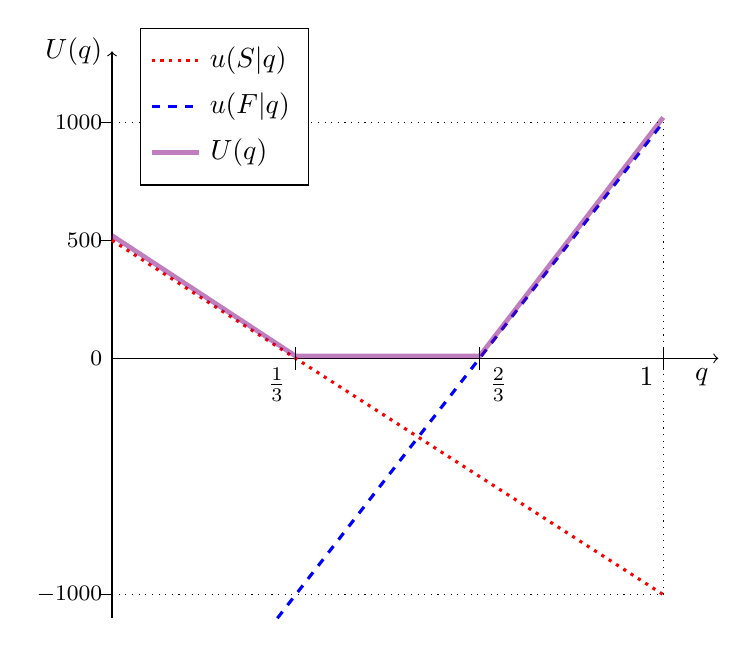
\begin{tikzpicture}[xscale=7,yscale=3]
			\draw[->] (0,0) -- (1.1,0) node[below left]{$q$};
			\draw[->] (0,-1.1) -- (0,1.3) node[left]{$U(q)$};
			\draw (0,0) node[left]{\footnotesize $0$};
			
			% Plot
			\draw[line width=0.4mm, red, dotted] (0,0.5) -- (1,-1);
			\draw[line width=0.4mm, blue, dashed] (0.3,-1.1) -- (1,1);
			\draw[line width=0.6mm, violet, opacity=0.5] (0,0.52) -- (0.333,0.01) -- (0.667,0.01) -- (1,1.02);
			
			% Ticks
			% x axis
			\draw (0.333,0) coordinate(q1) node[below left]{$\frac{1}{3}$};
			\draw (q1) ++(0,-0.05) -- ++(0,0.1);
			
			\draw (0.667,0) coordinate(q2) node[below right]{$\frac{2}{3}$};
			\draw (q2) ++(0,-0.05) -- ++(0,0.1);
			
			\draw (1,0) coordinate(q3) node[below left]{$1$};
			\draw (q3) ++(0,-0.05) -- ++(0,0.1);
			\draw[dotted] (1,-1) -- (1,1);
			
			% y axis
			\draw (0,0.5) coordinate(u1) node[left]{\footnotesize $500$};
			\draw (u1) ++(-0.02,0) -- ++(0.02,0);
			
			\draw (0,1) coordinate(u2) node[left]{\footnotesize $1000$};
			\draw (u2) ++(-0.02,0) -- ++(0.02,0);
			\draw[dotted] (u2) -- ++(1,0);
			
			\draw (0,-1) coordinate(u3) node[left]{\footnotesize $-1000$};
			\draw (u3) ++(-0.02,0) -- ++(0.02,0);
			\draw[dotted] (u3) -- ++(1,0);
			
			%Legend
			\matrix [draw, fill=white, below right] at (0.05,1.4) {
				\draw [line width=0.4mm, red, dotted] ++(-0.3,0) -- ++(0.6,0) node[black,right] {$u(S|q)$}; \\
				\draw [line width=0.4mm, blue, dashed] ++(-0.3,0) -- ++(0.6,0) node[black,right] {$u(F|q)$}; \\
				\draw [line width=0.6mm, violet, opacity=0.5] ++(-0.3,0) -- ++(0.6,0) node[black,right,opacity=1] {$U(q)$}; \\
			};
			\end{tikzpicture}
			\caption{$U(q)$}
			\label{fig:U}
		}
		\parbox{0.5\linewidth}{
			\centering
			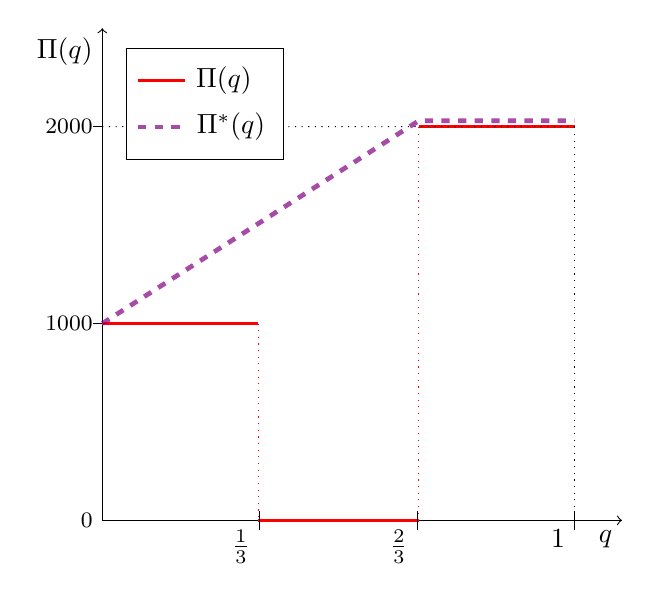
\begin{tikzpicture}[xscale=6,yscale=2.5,
			piline/.style={line width=0.4mm, red}
			]
			\draw[->] (0,0) -- (1.1,0) node[below left]{$q$};
			\draw[->] (0,0) -- (0,2.5) node[below left]{$\Pi(q)$};
			\draw (0,0) node[left]{\footnotesize $0$};
			
			% Plot
			% Pi
			\draw[piline] (0,1) -- (0.33,1);
			\draw[red,dotted] (0.33,1) -- (0.33,0);
			\draw[piline] (0.33,0) -- (0.67,0);
			\draw[red,dotted] (0.67,0) -- (0.67,2);
			\draw[piline] (0.67,2) -- (1,2);
			
			\draw[line width=0.6mm, violet, opacity=0.7, dashed] (0,1) -- (0.67,2.03) -- (1,2.03);
			
			% Ticks
			% x axis
			\draw (0.333,0) coordinate(q1) node[below left]{$\frac{1}{3}$};
			\draw (q1) ++(0,-0.05) -- ++(0,0.1);
			
			\draw (0.667,0) coordinate(q2) node[below left]{$\frac{2}{3}$};
			\draw (q2) ++(0,-0.05) -- ++(0,0.1);
			
			\draw (1,0) coordinate(q3) node[below left]{$1$};
			\draw (q3) ++(0,-0.05) -- ++(0,0.1);
			\draw[dotted] (1,0) -- (1,2);
			
			% y axis
			\draw (0,1) coordinate(u1) node[left]{\footnotesize $1000$};
			\draw (u1) ++(-0.02,0) -- ++(0.02,0);
			
			\draw (0,2) coordinate(u2) node[left]{\footnotesize $2000$};
			\draw (u2) ++(-0.02,0) -- ++(0.02,0);
			\draw[dotted] (u2) -- (1,2);
			
			%Legend
			\matrix [draw, fill=white, below right] at (0.05,2.4) {
				\draw [piline] ++(-0.3,0) -- ++(0.6,0) node[black,right] {$\Pi(q)$}; \\
				\draw [line width=0.6mm, violet, opacity=0.7, dashed] ++(-0.3,0) -- ++(0.6,0) node[black,right,opacity=1] {$\Pi^*(q)$}; \\
			};
			\end{tikzpicture}
			\caption{$\Pi(q)$ and $\Pi^*(q)$}
			\label{fig:profit}
		}
	\end{figure}

	\begin{enumerate}
		\item The consumer's utilities from the three options are given by:
		\begin{align*}
			u(F|q) &= q \cdot 3000 + (1-q) \cdot 0 - 2000 \\
			u(S|q) &= q \cdot 0 + (1-q) \cdot 1500 - 1000 \\
			u(\varnothing|q) &= 0
		\end{align*}
		The three are depicted in Figure \ref{fig:U}.
		Taking the maximum of the three for a given $q$ yields the optimal choice rule
		\begin{equation*}
			a(q) = 
			\begin{cases}
			F & \text{ if } q \geq \frac{2}{3}; \\
			\varnothing & \text{ if } q \in \left[ \frac{1}{3}, \frac{2}{3} \right]; \\
			S & \text{ if } q \leq \frac{1}{3}.
			\end{cases}
		\end{equation*}
		\item From the previous answer, we get
		\begin{equation*}
			U(q) = 1000 \cdot 
			\begin{cases}
			3q - 2 & \text{ if } q \geq \frac{2}{3}; \\
			0 & \text{ if } q \in \left[ \frac{1}{3}, \frac{2}{3} \right]; \\
			0.5 - 1.5q & \text{ if } q \leq \frac{1}{3}.
			\end{cases}
		\end{equation*}
		\item From (1), we have
		\begin{equation*}
			\Pi(q) = 1000 \cdot 
			\begin{cases}
			2 & \text{ if } q \geq \frac{2}{3}; \\
			0 & \text{ if } q \in \left[ \frac{1}{3}, \frac{2}{3} \right]; \\
			1 & \text{ if } q \leq \frac{1}{3}.
			\end{cases}
		\end{equation*}
		\item As suggested by the hint, look at the graph of $\Pi(q)$ depicted in Figure \ref{fig:profit}.
		The profit $\Pi^*(q)$ that the seller can achieve under the optimal Bayesian Persuasion mechanism is given by the smallest concave envelope of $\Pi(q)$. You can see from the Figure that $\Pi^*(q)$ coincides with $\Pi(q)$ for $q \in NP \equiv \{0\} \cup [2/3,1]$ -- if the consumer's prior belonged to this set then no persuasion mechanism could increase the seller's profit. For any remaining prior (which includes our case, $q_0=1/2$), the optimal persuasion mechanism splits the prior between two closest points in $NP$. In case of prior $q_0 = 1/2$, the optimal persuasion mechanism prescribes posteriors $q_1 = 0$ and $q_2 = 2/3$. The probabilities of these posteriors can then be computed from the consistency requirement (a.k.a. law of total probability):
		\begin{align*}
			\tau_1 \cdot q_1 + \tau_2 \cdot q_2 &= q_0
			\\
			\Leftrightarrow \tau_1 \cdot 0 + \tau_2 \cdot \frac{2}{3} &= \frac{1}{2}
		\end{align*}
		and the requirement $\tau_1 + \tau_2 = 1$. The two together yield $(\tau_1,\tau_2) = (1/4, 3/4)$. Hence the optimal experiment $Q$ induces posterior $q_1 = 0$ with probability $\tau_1 = 1/4$ and posterior $q_2 = 2/3$ with probability $\tau_2 = 3/4$.
		
		Note: graph in Figure \ref{fig:profit_wrong} is \textbf{not} considered correct (since the resulting $\Pi^*(q)$ is not concave).
	\end{enumerate}

	\begin{figure}
		\centering
		\begin{tikzpicture}[xscale=6,yscale=2.5,
		piline/.style={line width=0.4mm, red}
		]
		\draw[->] (0,0) -- (1.1,0) node[below left]{$q$};
		\draw[->] (0,0) -- (0,2.5) node[below left]{$\Pi(q)$};
		\draw (0,0) node[left]{\footnotesize $0$};
		
		% Plot
		% Pi
		\draw[piline] (0,1) -- (0.33,1);
		\draw[red,dotted] (0.33,1) -- (0.33,0);
		\draw[piline] (0.33,0) -- (0.67,0);
		\draw[red,dotted] (0.67,0) -- (0.67,2);
		\draw[piline] (0.67,2) -- (1,2);
		
		\draw[line width=0.6mm, violet, opacity=0.7, dashed] (0,1.03) -- (0.33,1.03) -- (0.67,2.03) -- (1,2.03);
		
		% Ticks
		% x axis
		\draw (0.333,0) coordinate(q1) node[below left]{$\frac{1}{3}$};
		\draw (q1) ++(0,-0.05) -- ++(0,0.1);
		
		\draw (0.667,0) coordinate(q2) node[below left]{$\frac{2}{3}$};
		\draw (q2) ++(0,-0.05) -- ++(0,0.1);
		
		\draw (1,0) coordinate(q3) node[below left]{$1$};
		\draw (q3) ++(0,-0.05) -- ++(0,0.1);
		\draw[dotted] (1,0) -- (1,2);
		
		%Legend
		\matrix [draw, fill=white, below right] at (0.05,2.4) {
			\draw [piline] ++(-0.3,0) -- ++(0.6,0) node[black,right] {$\Pi(q)$}; \\
			\draw [line width=0.6mm, violet, opacity=0.7, dashed] ++(-0.3,0) -- ++(0.6,0) node[black,right,opacity=1] {$\Pi^*(q)$}; \\
		};
		\end{tikzpicture}
		\caption{Incorrect $\Pi^*(q)$}
		\label{fig:profit_wrong}
	\end{figure}
	\fi
\end{ex}



%%-----------------------------------------------------------------------------------------------------
\end{document}